\begin{itemize}
  \item[] \centering\large\textsc{\underline{System Architecture:}}\\\normalsize\texttt{Top Level}
  \begin{itemize}
    \item[] 
    \begin{tikzpicture}
      \umlusecase[x=5]{CS Major}
      \umlusecase[x=5,y=-2]{English Major}
      \umlactor{Student}
    \end{tikzpicture}
  \end{itemize}
\end{itemize}
\clearpage
\begin{itemize}
  \item[] \centering\large\textsc{\underline{System Architecture:}}\\\normalsize\texttt{Low Level}
  \begin{itemize}
    \item[] 
    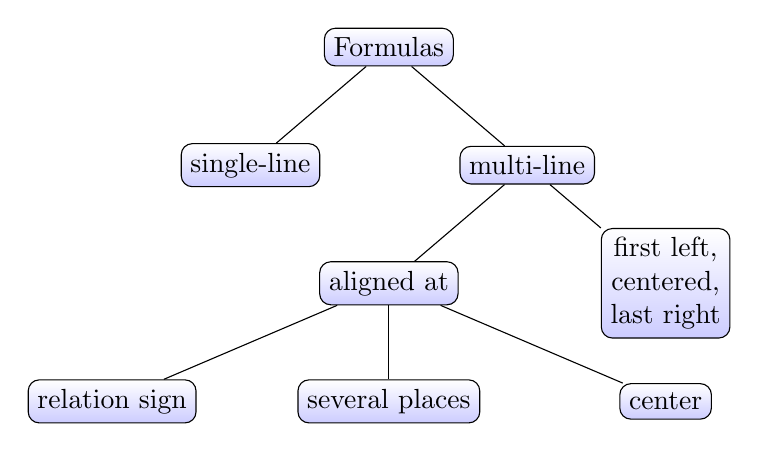
\begin{tikzpicture}[sibling distance=10em,
      every node/.style = {shape=rectangle, rounded corners,
        draw, align=center,
        top color=white, bottom color=blue!20}]]
      \node {Formulas}
        child { node {single-line} }
        child { node {multi-line}
          child { node {aligned at}
            child { node {relation sign} }
            child { node {several places} }
            child { node {center} } }
          child { node {first left,\\centered,\\last right} } };
    \end{tikzpicture} 
  \end{itemize}
\end{itemize}
\clearpage